%%%%%%%%%%%%%%%%%%%%%%%%%%%%%%%%%%%%%%%%%%%%%%%%%%%
%% P3: Phenomenology of Particle Physics                         
%%
%% Author:  André Rubbia                   		 
%%
%% Figure 23.9 Decay electron/positron energy distribution for different values of the Michel parameter $\rho$.
%%
%% This work is licensed under the Creative Commons Attribution 4.0 International License. 
%% To view a copy of this license, visit http://creativecommons.org/licenses/by/4.0/ or 
%% send a letter to Creative Commons, PO Box 1866, Mountain View, CA 94042, USA.
%%
%%%%%%%%%%%%%%%%%%%%%%%%%%%%%%%%%%%%%%%%%%%%%%%%%%%

\documentclass[a4paper,10pt]{article}

\usepackage[T1]{fontenc}
\usepackage[utf8]{inputenc}
\usepackage{lmodern}
\usepackage[labelfont=bf]{caption}
\usepackage{upgreek}

\usepackage{tikz}
\usepackage{pgfplots}
\pgfplotsset{compat=1.17}
\usepgfplotslibrary{ternary}
\usepgfplotslibrary{fillbetween}
\usepgfplotslibrary{external}

\def\d{\mathrm{d}}
\setlength{\oddsidemargin}{-1.0cm}
\setlength{\evensidemargin}{-1.0cm}
\setlength{\textheight}{25cm}
\setlength{\textwidth}{18cm}

\begin{document}

%%%%%%%%%%%%%%%%   FIGURE  %%%%%%%%%%%%%%%%%%%%%%%%%%%%%%
\begin{figure}[htb]
	\centering
\begin{tikzpicture}[scale=1.]
\begin{axis}[xmin=0, xmax=1,
	xtick={0,0.5,1},
	ymin=0, ymax=1.5,
	title=$\mu^\pm\rightarrow e^\pm\nu\bar\nu$,
	xlabel=Reduced energy $x$,
	ylabel=Relative decay rate,
	xmajorgrids=true,
	ymajorgrids=true,
	legend entries={$\rho=3/4$,$\rho=0$,$\rho=1$},
	legend pos = north west]
	\addplot[domain=0:1,blue,very thick] {2*x^2*(3*(1-x)+2*(3/4)/3*(4*x-3))};
	\addplot[domain=0:1,magenta,dashed,very thick] {2*x^2*(3*(1-x)+2*(0)/3*(4*x-3))};
	\addplot[domain=0:1,red,dotted,very thick] {2*x^2*(3*(1-x)+2*(1)/3*(4*x-3))};
\end{axis}
\end{tikzpicture}
\caption{Decay electron/positron energy distribution for different values
of the Michel parameter $\rho$.}
\end{figure}
%
%%%%%%%%%%%%%%%%   END FIGURE  %%%%%%%%%%%%%%%%%%%%%%%%%%%%%%
%
\end{document}
